\setlength{\footskip}{8mm}

\chapter{METHODOLOGY}\label{methodology}

\section{Study 1: Confirming the parameters}\label{metho-s1}

The purpose of this study is to clarify how measurement sites and schemes affect Raman spectra.
The outcome of this study will be used to design the experiment in Section~\ref{metho-s2}.

\subsection{Equipment}
The Raman instrument equipped with a 785 nm laser and 10x objective lens will be used to assess the Raman spectra.
The Accu-Chek® Guide Meter is representing a standard blood glucose meter for SMBG \citep{accu2022} and will be used for assessing glycemic.

\subsection{Studying Measuring schemes}
We will evaluate the Raman spectroscopy at four measurement sites: the wrist, forearm, index fingertip, and index nail fold.
The measuring schemes will be put to the test to see which one produces the strongest scattering signal without introducing a fluorescence interference.
The optimal measuring schemes will be used for the rest of the Raman scattering assessment.

\subsection{Data collection}
The Oral Glucose tolerance Test (OGTT) will be used to manipulate glycemic of the three healthy participants.
The participants have to conduct fasting at least eight hours before the test.
Once the participants arrived at the experiment area, they will be instructed to acclimate for 30 minutes.
During the acclimation, instructor will repeat the experiment procedure.
Both Raman Instrument and conventional SMBG equipment will be used to collect data at the interested measuring site.
When the acclimation is completed, the first sample will be drawn.
The participants begin the OGTT by consume a 250 ml of water containing 75 g of glucose in five minutes.
Then, for the next two hours;
(1) collecting Raman spectra at the interested measuring site every five minutes;
(2) collecting blood sample at the interested measuring site every 20 minutes.
In total, there will be 25 Raman samples and eight blood samples.

Each participant has to repeat the experiment until all four measuring sites are measured. 
The experiment has to be done on another day.

\subsection{Metric}

The subtraction of two Raman signals will be used to extract the glucose fingerprint.
The remaining signal is the change of glucose concentration as showed in the following derivation.

The Raman spectra ($\text{RS}$) contains glucose fingerprint ($\text{G}$) and tissue spectra ($\text{T}$).

\begin{equation}\label{eq:rs}
    \text{RS} = \text{G} + \text{T}
\end{equation}

Then, the subtraction of two Raman signal can be represented as follows;

\begin{equation}\label{eq:deltars}
    \Delta \text{RS} = \text{RS}_1 - \text{RS}_2
\end{equation}

where $\text{RS}_i$ is the Raman spectra measured at time $i$. 
Then, substituting Equation~\ref{eq:deltars} with Equation~\ref{eq:rs} will derive the follows

\begin{equation}
    \Delta \text{RS} = \Delta \text{G} + \Delta \text{T}
\end{equation}

Given the measuring site is the same, the tissue spectra will also be the same. 
Thus, $\Delta \text{T}$ is $0$.
Then, it is obvious that 

\begin{equation}
    \Delta \text{RS} = \Delta \text{G}
\end{equation}

Therefore, the best measuring site is the one that produces the greatest correlation between $\Delta \text{G}$ and the actual changes in blood glucose.

%%%%%%%%%%%%%%%%%%%%%%%%%%%%%%%%%%%%%%%%%%%%%%%%%%%%%%%%%%%%%%%%%%%%%%%%%%%%%
\section{Study 2: Raman scattering of blood glucose study}\label{metho-s2}

The purpose of this study is to model the relationship between Raman spectra and blood glucose.
The same equipment from Section~\ref{metho-s1} will be used.
The measuring site and scheme are chosen based on the result of Section~\ref{metho-s1}.

\section{Data Collection}

The same data collection and experiment procedure from Section~\ref{metho-s1} will also be used.
In this study, we increase the number of participants to 15 participants.
The participants shall be from three different age groups (5 each from 20 to 35 years, 36 to 50 years, and 51 to 65 years).

A total of $15 \times 25 =  375$ Raman samples and $15 \times 8 = 120$ blood samples are collected.

\section{Preprocessing and Data Modeling}

The acquired Raman spectra will be normalized by their intensity of 1450 or 1549 $\text{cm}^{-1}$.
Thus, there are three preprocessing options: (1) without normalization, (2) normalize with 1450 $\text{cm}^{-1}$, and (3) normalized with 1549 $\text{cm}^{-1}$.
The Linear Regression (LR) model will be used to assess the linearity of 1125 $\text{cm}^{-1}$ with glucose concentration.
The MLR model with 911, 1060, 1125 $\text{cm}^{-1}$ as inputs we will use for multivariate analysis.
As a baseline model, full spectrum with PLS will also be employed.

In total, there will be $3 \times 3 = 9$ combinations to compare.

\section{Metric}

The model performance will be assessed using the Pearson correlation.
Additionally, resource usage during prediction will be tracked.

\section{Study 3: Designing and developing wearable blood glucose device}

\begin{figure}
    \caption{An example of wearable \citep{applewatch}.}
    \centerline{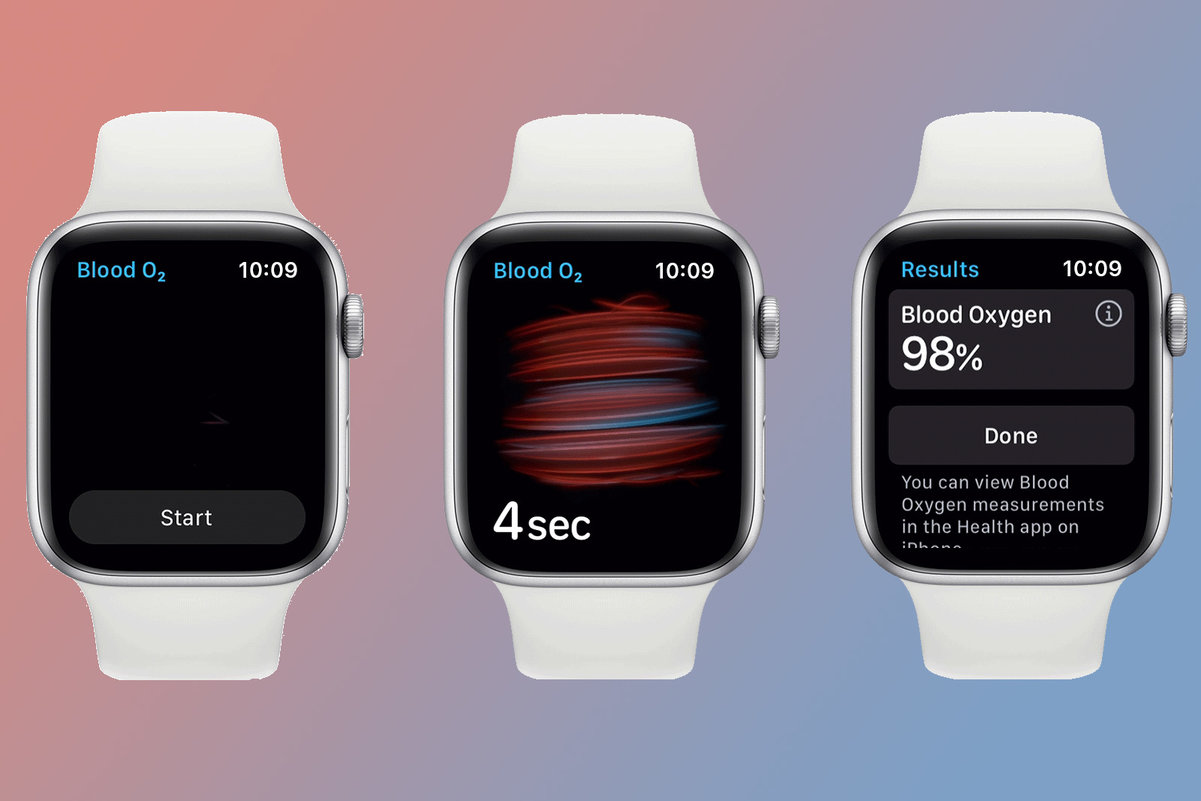
\includegraphics[width=3in]{figures/example-wearable-applewatch.jpg}}\label{fig:applewatch}
    % \small{\textit{Note.} Additional notes goes here.}
\end{figure}


\textbf{Objective}: Design and develop a prototype of a wearable SMBG.\\
% \textbf{Independent Variables}: \\
% \textbf{Dependent Variables}: \\
\textbf{Outcome}: A prototype.

\section{Study 4: Device Evaluation}

\textbf{Objective}: To evaluate the prototype, we redo Section~\ref{metho-s2} experiment with our prototype.\\
\textbf{Independent Variables}: Raman scattering of blood\\
\textbf{Dependent Variables}: Glycemic\\
\textbf{Outcome}: Prototype achieves glycemic prediction correlation $R^2 > 0.8$ with actual glycemic.